%% This is a tikz file

% This file is set up to use 11pt palatino font.
\tikzset{node lower left/.style={font=\scriptsize,anchor=north east,yshift=-0.032cm,text height=0.198cm,text depth=0.079cm,inner sep=0.03cm},
leaf/.style={font=\normalsize,anchor=west,text height=0.271cm,text depth=0.109cm,inner sep=0.13cm},
node upper left/.style={font=\scriptsize,anchor=south east,yshift=-0.032cm,text height=0.198cm,text depth=0.079cm,inner sep=0.03cm},
bracket label/.style={font=\normalsize,anchor=west,text height=0.271cm,text depth=0.109cm,inner sep=0.2cm},
node upper right/.style={font=\scriptsize,anchor=south west,text height=0.198cm,text depth=0.079cm,inner sep=0.03cm},
node right/.style={font=\scriptsize,anchor=west,text height=0.198cm,text depth=0.079cm,inner sep=0.03cm},
branch/.style={font=\tiny,text height=0.149cm,text depth=0.059cm,inner sep=0.025cm},
root/.style={font=\normalsize,anchor=east,text height=0.271cm,text depth=0.109cm},
node lower right/.style={font=\scriptsize,anchor=north west,text height=0.198cm,text depth=0.079cm,inner sep=0.03cm}}
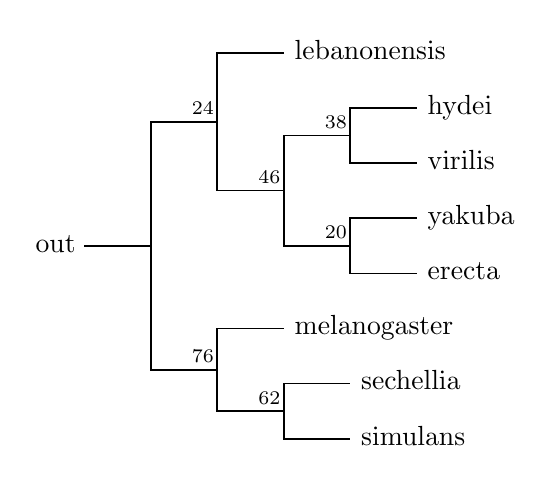
\begin{tikzpicture}[semithick,inner sep=0.1cm]
%                          +---------8:lebanonensis
%                          |
%               +----------7:24                +----------11:hydei
%               |          |         +---------10:38
%               |          |         |         +----------12:virilis
%               |          +---------9:46
%               |                    |         +----------14:yakuba
% out:6---------5                    +---------13:20
%               |                              +----------15:erecta
%               |
%               |          +---------1:melanogaster
%               +----------0:76
%                          |         +---------3:sechellia
%                          +---------2:62
%                                    +---------4:simulans

% The scale is 8.442000, and the yScale is 0.700000

%% Coordinates of nodes.
\coordinate (n6) at (0.000,2.450);
\coordinate (n5) at (0.844,2.450);
\coordinate (n5p) at (0.000,2.450);
\coordinate (n7) at (1.688,4.025);
\coordinate (n7p) at (0.844,4.025);
\coordinate (n8) at (2.533,4.900);
\coordinate (n8p) at (1.688,4.900);
\coordinate (n9) at (2.533,3.150);
\coordinate (n9p) at (1.688,3.150);
\coordinate (n10) at (3.377,3.850);
\coordinate (n10p) at (2.533,3.850);
\coordinate (n11) at (4.221,4.200);
\coordinate (n11p) at (3.377,4.200);
\coordinate (n12) at (4.221,3.500);
\coordinate (n12p) at (3.377,3.500);
\coordinate (n13) at (3.377,2.450);
\coordinate (n13p) at (2.533,2.450);
\coordinate (n14) at (4.221,2.800);
\coordinate (n14p) at (3.377,2.800);
\coordinate (n15) at (4.221,2.100);
\coordinate (n15p) at (3.377,2.100);
\coordinate (n0) at (1.688,0.875);
\coordinate (n0p) at (0.844,0.875);
\coordinate (n1) at (2.533,1.400);
\coordinate (n1p) at (1.688,1.400);
\coordinate (n2) at (2.533,0.350);
\coordinate (n2p) at (1.688,0.350);
\coordinate (n3) at (3.377,0.700);
\coordinate (n3p) at (2.533,0.700);
\coordinate (n4) at (3.377,0.000);
\coordinate (n4p) at (2.533,0.000);

%% horizontal lines
\draw (n5p) -- (n5);
\draw (n7p) -- (n7);
\draw (n8p) -- (n8);
\draw (n9p) -- (n9);
\draw (n10p) -- (n10);
\draw (n11p) -- (n11);
\draw (n12p) -- (n12);
\draw (n13p) -- (n13);
\draw (n14p) -- (n14);
\draw (n15p) -- (n15);
\draw (n0p) -- (n0);
\draw (n1p) -- (n1);
\draw (n2p) -- (n2);
\draw (n3p) -- (n3);
\draw (n4p) -- (n4);

%% vertical lines
\draw [line cap=rect] (n7p) -- (n0p);
\draw [line cap=rect] (n8p) -- (n9p);
\draw [line cap=rect] (n10p) -- (n13p);
\draw [line cap=rect] (n11p) -- (n12p);
\draw [line cap=rect] (n14p) -- (n15p);
\draw [line cap=rect] (n1p) -- (n2p);
\draw [line cap=rect] (n3p) -- (n4p);

%% leaf labels
\node [leaf,text height=0.271cm,text depth=0.109cm] at (n8) {lebanonensis};
\node [leaf,text height=0.271cm,text depth=0.109cm] at (n11) {hydei};
\node [leaf,text height=0.271cm,text depth=0.109cm] at (n12) {virilis};
\node [leaf,text height=0.271cm,text depth=0.109cm] at (n14) {yakuba};
\node [leaf,text height=0.271cm,text depth=0.109cm] at (n15) {erecta};
\node [leaf,text height=0.271cm,text depth=0.109cm] at (n1) {melanogaster};
\node [leaf,text height=0.271cm,text depth=0.109cm] at (n3) {sechellia};
\node [leaf,text height=0.271cm,text depth=0.109cm] at (n4) {simulans};

%% root label
\node [root,text height=0.271cm,text depth=0.109cm] at (n6) {out};

% internal node labels (doSmartLabels is True)
\node [node upper left,text height=0.198cm,text depth=0.079cm] at (n7) {24};
\node [node upper left,text height=0.198cm,text depth=0.079cm] at (n9) {46};
\node [node upper left,text height=0.198cm,text depth=0.079cm] at (n10) {38};
\node [node upper left,text height=0.198cm,text depth=0.079cm] at (n13) {20};
\node [node upper left,text height=0.198cm,text depth=0.079cm] at (n0) {76};
\node [node upper left,text height=0.198cm,text depth=0.079cm] at (n2) {62};

\end{tikzpicture}
